\documentclass[conference]{IEEEtran}

\ifCLASSINFOpdf
   \usepackage[pdftex]{graphicx}
  % declare the path(s) where your graphic files are
   \graphicspath{{./png/}}
  % and their extensions so you won't have to specify these with
  % every instance of \includegraphics
   \DeclareGraphicsExtensions{.png}
\else
  % or other class option (dvipsone, dvipdf, if not using dvips). graphicx
  % will default to the driver specified in the system graphics.cfg if no
  % driver is specified.
  % \usepackage[dvips]{graphicx}
  % declare the path(s) where your graphic files are
  % \graphicspath{{../eps/}}
  % and their extensions so you won't have to specify these with
  % every instance of \includegraphics
  % \DeclareGraphicsExtensions{.eps}
\fi

% correct bad hyphenation here
\hyphenation{op-tical net-works semi-conduc-tor}


\begin{document}

\title{Robust Energy-Aware Routing with Uncertain Traffic Demands}


\author{\IEEEauthorblockN{Heng Lin}
\IEEEauthorblockA{Tsinghua University}
\and
\IEEEauthorblockN{Mingwei Xu}
\IEEEauthorblockA{Tsinghua University}
\and
\IEEEauthorblockN{Yuan Yang}
\IEEEauthorblockA{Tsinghua University}}


% make the title area
\maketitle

% As a general rule, do not put math, special symbols or citations
% in the abstract
\begin{abstract}
Energy conservation has become a major challenge to the Internet. In existing approaches, a part of line cards 
are switched into sleep mode for energy conservation, and the routing is configured carefully to balance energy saving 
and traffic engineering goals, such as the maximum link utilization ratio (MLUR). Typically, traffic demands are 
used as inputs, and routing is computed accordingly. However, accurate traffic matrices are difficult to obtain and 
are changing frequently. This makes the approaches difficult to implement. Further, the routing may shift 
frequently, and is not robust to sudden traffic changes.

In this paper, we propose a different approach that finds one energy-aware routing robust to a set of traffic 
matrices, in particular, to arbitrary traffic demands. Such a routing without energy consideration is known as 
the demand-oblivious routing, and is well studied. However, the problem becomes much more challenging when energy 
conservation is involved. To overcome the challenges, we first define a new metric, namely oblivious performance 
ratio with energy constraint, which reflects the MLUR distance from a routing to the optimal routing when 
certain energy conservation requirement is satisfied. We model the problem of minimizing the performance ratio, 
and analyze the lower and the upper bounds. Then, we propose Robust Energy-Aware Routing (REAR) to solve 
the problem in two phases. REAR select sleeping links based on extended algebraic connectivity, and compute the 
routing based on a classical demand-oblivious routing algorithm. We evaluate our algorithms on real and 
synthetic topologies. The simulation results show that REAR can save XX\% of line card power while the performance 
ratio is less than XX.
\end{abstract}

\IEEEpeerreviewmaketitle

\section{Introduction}
We aim to find the ``robust'' route for all possible traffic matrix, not only consider performance but also energy 
consumption in network.

\section{Motivation}
Suppose two hosts named host A and host B, and there are three links between 
them, respectively, capacity with 2M, 3M and 5M. Now demands come, with 1M from A to B. we regard the capacity 
as the power of the link, and the minimum maximum utilization of network links as a metric of the network performance. 
There are two directions for operating this example. One consider the min power consumption except for the 
utilization, it is obviously that we should close the larger power consuming links, such as the 5M and 3M links, and 
all the traffic go through the 2M link. In this way, the min max utilization of network is 0.5 and the power consuming 
is 2 units (means the power difference come from the link mainly). The other consider the power except for the 
utilization reversely, so we should split the 1M traffic to three parts, 0.2M across 2M link, 0.3M across 3M link and 
0.5M across 5M, consequently with a min max utilization of 0.1, but the power is 10 units however.

Two directions mentioned above both are extremely single-consideration. Previous researchers solve the problem more 
considerable, include ``GreenTE'' and ``a\%-green is engouh''. The former set a threshold of min max utilization, 
close links as many as possible to achive the most power saving. And the latter one set a destination of the power 
saving, calculate optimal route for get the min max utilization. Two work have their restriction, which both need a 
specific traffic matrix that as base of their optimization.

But the need of precise current traffic matrix shound be carefully checked. Although some researcher contribute to this 
area, the real precise traffic matrix still be a challenge. Take a step back, the dynamic of traffic matrix is more 
diffcult even if we obtain the precise current one. Futhermore, ISP will not want to change their route policy 
frequently, as it will result in other route failure possiblly. So our question is that : Is there exist a route both 
satisfy power and utilization requirement for any traffic matrix given?


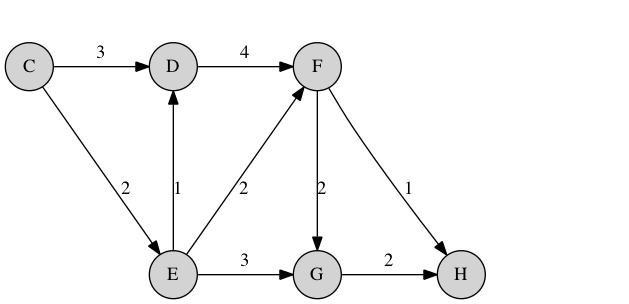
\includegraphics[width=10cm]{net5}


David Applegate propose a method for obtain a route wihich is ``robust'' to variations in demands for a specific network topology. 

\section{Model}
We model the network as a undirected graph $G = (V, E)$, where $V$ is the set of vertices (i.e., routers and end hosts), 
and $E$ is the set of links (either link between routers or router and end-host). In graph $G$, two vertices $u$ and $v$
are called connected if $G$ contains a path from $u$ to $v$. Then We say graph $G$ is connected, if and only if 
every pair of vertices in the graph is connected.

Let $\theta(G) = \{ (V, E - \{ e \}) | e \in E \}$ denote the network set after closing/removing the link $e$ from
$G$. Then, choosing the connected graph from $\theta(G)$ to consist a new set, denoted by 
$\Theta(G) = \{G | G \in \theta(G) \& \& G is connected\}$. We call $\Theta(G)$ as successor of $G$.

A $traffic matrix$ (abbreviation as TM below) is the set of traffic of each Origin-Destination(OD) pair in 
network $G$, and a $routing$ specifies how traffic of each OD pair is routed across the network. Usually, there are 
multiple paths for each OD pair and each path routes a fraction of the traffic. Let $m$ denote the $traffic matrix$, 
which can be represented by a set of trinary group like $(a, b, d_{ab}$, where $a$ and $b$ is the origin and 
destination of pair respectively, $d_{ab}$ is the traffic demand of the OD pair. 

Let $r$ denote the $routing$ mentioned above, which is specified by a set of values $f_{ab}(i,j)$ that specifies the 
fraction of demand from $a$ to $b$ that is routed on the link $(i,j)$. So an OD pair contribute to the traffic of 
link $(i,j)$ is $d_{ab}f_{ab}(i,j)$, and all the traffic across link $(i,j)$ can be calculated as :
\begin{equation}
	\sum_{(a,b,d_{ab}\in m)} d_{ab}f_{ab}(i,j)
\end{equation}

Futhermore, we define the utilization of link as traffic acorss the link divide capacity of the link, as ;
\begin{equation}
	u_{ij} = \frac{\sum_{a,b} d_{ab}f_{ab}(i,j)}{cap_{ij}}
\end{equation}
where $cap_{ij}$ si the capacity of the link $(i,j)$.

A common metric for the performance of a given routing with respect to a certain TM is the $maximum link utilization$.
This is the maximum utilization of link over all ones, Formally, the maximum link utilization of a routing $r$ on 
TM $m$ in network $G(V,E)$ is 
\begin{equation}
	U_{r, m, G} = \max_{(i,j)\in E} u_{ij}
\end{equation}

The $optimal routing$ in all the possible route $R$ for network $G$ is a routing which minimize the maximum utilization,
the minimum maximum utilization is called optimal utilization, can be represented by :
\begin{equation}
	OptU_{m, G} = \min_{r\in R} U_{r, m, G}
\end{equation}

The $performance ratio$ of a given routing $r$ on a given TM $m$ and a given network $G$ meaures how far from being 
optimal, it is defined as the maximum link utilization divided by optimal utilization on the $m$ and $G$, as following : 
\begin{equation}
	P(\{ r \},\{ m \}, G) = \frac{U_{r,m,G}}{OptU_{m,G}}
\end{equation}

We now extend the definition of performance ratio of a routing to be with respect to a set of TMs $M$. 
\begin{equation}
	P(\{ r \}, M, G) = \max_{m\in M} P(\{ r \}, \{ m \}, G)
\end{equation}

Obviously, the optimal routing in routing set $R$ for the set of TMs is a routing which minimize the extended 
performance ratio, such as :
\begin{equation}
	P(R, M, G) = \min_{r\in R} P(\{ r \}, M, G)
\end{equation}

I.E. the routing $r$ which arrive at the value of $P(R,M,G)$ is the most ``robust'' routing for the TM set $M$ 
in the network $G$, and if the $M$ range enough, we say that the ``robust'' routing is independent of specific TM.

But definition of ``robust'' above will not work well for next situation. Let us take a cycle network topology $C$ as 
an simple example, in which we should choose one link to close. Before link cutting, the $P(R, M, C)$ is 
approximate to 2, but no matter which link is chosen to close, the cycle network will change to a line network $L$. 
Obviously, the $P(R, M, L)$ will always equal to 1. It means that there is no difference from removing which link,
But the contradiction here is that, the choice for which link should be removed is really different because the 
links are not always the same with each other, such as their capacity.

The reason for the ``fake robust'' is that, the routing in the successor graph (i.e. $L$ in above example) become 
unique, the current routing always be the optimal routing. More generally, we should make a little modification
for the $performance ratio$ as the network self changes.

Let $G$ be the origin network, and the $G^* \in \Theta(G)$ be the successor network from $G$ after closing/removing
some link, we define $performance ratio between different graphs$ as the performance ratio of successor graph divide 
the optimal performance ratio of father graph, like :
\begin{equation}
	P(R^*, \{ m\}, G, G^*) = \min_{r \in R^*} \frac{U_{r,m,G^*}}{OptU_{m,G}}
\end{equation}
where $R^*$ is the routing set on network $G^*$.

And question is that how to meaure a successor network topology is ``robust'' enough for the TM set $M$ when 
pruning is proceeding. We consider the worst situation, namely the successor network topology has its maximum
performance ratio when the TM is $m \in M$, described as following :
\begin{equation}
	P(R^*, M, G, G^*) = \max_{m \in M} P(R^*, \{ m \}, G, G^*)
\end{equation}

Now we can say that, if a successor network arrive the minimum performance ratio, it is the ``robust'' successor 
network graph. Formally, we define the performance ratio as $optimal successor performance ratio$ :
\begin{equation}
	P^{*}(M, G) = \min_{G^* \in \Theta(G)} P(R^*, M, G, G^*)
\end{equation}
where $M$ is the TM set, and $R^*$ is routing set. 

If the scope of $M$ is large engouh, the optimal successor network graph is alwo independent from specific TM. 

\subsection{Model Example}
We will take an example to explain how to choose the link to close in our experiment.
Three hostes include : A, B, C, Three links are with repectively capacity of 3M, 4M and 2M. For simpleness, we suppose 
there are two TM : ${(A,B,2M), (A,C,1M)}, {(A,B,1M), (A,C,1M)}$.For each traffic matrix, the optimal route is 
obvious, we will trace 2M from A to B across the lower link and trace the 1M from A to C across the upper one 
for the first traffic matrix, whose maximum link utilization is 0.5. we will trace all the traffic acorss the
lower link for the second traffic matrix, whose maximum link utilization is 0.5 as well.

Now for some reason, we will choose one link to shut down for power saving without lose connection of the network. 
There are two choice, remove either the upper link or the lower link. Let us take a little calculation: when 
remove the upper one, we should change all the traffic acorss the lower link, as a result, in the first  
TM the maximum link utilization is 0.75 and the second is 0.5; when close the lower link, we should trace all the 
traffic acorss the upper link, in the first TM the link utilization is 1 and the other is 0.667. 
So according to our theory, the $P^{*}(M, G)$ should be 1.5 and the optimal successor network topology will be
the one which 3M link is closed.

\section{Algorithm}
In our paper, Robust Energy-Aware Routing (REAR) algorithm works in two phases. Firstly, REAR select links 
should be sleeping from the origin topology based on extended algebraic connectivity, then compute the robust 
routing by demand-oblivious routing algorithm.


\subsection{Extend Algebraic Connectivity}
Network topology is represented by $G = (V, E)$ as mentioned in Model section, where $V$ is the set of vertices
and $E$ is the set of links. We say $A(G)$ is the Adjacency Matrix of graph $G$, that include information for which
vertices of the graph are adjacent to which other vertices. $A(G)$ is a $N \times N$ matrix, where
$N = |V|$ and non-diagonal entry $a_{ij}$ equal to the number of edges from vertex $i$ to vertex $j$, in this paper,
$a_{ij}$ always be 1 if $(i,j) \in E$ otherwise 0. And we stipulate the diagonal element $a_{ii}$ be 0.


We say $D(G)$ is the Degree Matrix of graph $G$, which is a diagonal matrix and diagonal entry $d_{ii}$ denote 
the degree of node $i$. It is obvious that there is $d_{ii} == \sum_{j} a_{ij}$.


Then we define Laplacian Matrix $L(G)$ of graph $G$ as the difference between Degree Matrix and Adjacency Matrix :
\begin{equation}
	L(G) = D(G) - A(G)
\end{equation}
where $D(G)$ is the Degree Matrix and $A(G)$ is the Adjacency Matrix.


In the mathematical field of graph theory, the number of eigenvalues equal to 0 is the number of connected 
componements of $G$, so the smallest eigenvalue always be 0. And we call the second smallest one as
algebraic connectivity, which is greater than 0 if and only if graph $G$ is connected. Further more,  
it measures the connectivity and stability of graph, the greater of which, the more connective of graph;
and it is a metric of average distance between any two vertices of graph $G$.


As far as we know, 
algebraic connectivity regard every link the same, without considering the capacity of each one, but it is 
ridiculous in network. It is easy to see, link with greater capacity is more important than the same one
with lower capacity. and in graph theory, algebraic connectivity value monotonically increased when we
increase the weight of link between vertices. So we extend the algebraic connectivity definition by following ways:

\begin{enumerate}
	\item We change the Adjacency Matrix from binary-matrix to float-matrix, i.e. if $(i,j) \in E$ we set the $a_{ij}$
with the capacity of link $l_{ij}$ instead of binary value 1.
	\item Degree Matrix is not ever the denotation for the degree of nodes, but the conbined capacity of all the links
adjacent to the node, there is still exist the equation: $d_{ij} == \sum_{j} a_{ij}$
	\item No modification for definition of Laplacian Matrix
\end{enumerate}


We calculate new extend algebraic connectivity from the new Laplacian matrix, denoted by $\lambda_2(G)$.


Topology always have different extend algebraic connectivity values, it is clear that when one link is added or 
removed from the graph, the extend algebraic connectivity value changes accordingly. And we say the changed value
is the impact of this link on the graph. Supposed we sleep link $l$ from graph $G$, new graph is described as $G^*$, 
we defined the impact of link $l$ as :
\begin{equation}
	\Delta_l = \lambda_2(G) - \lambda_2(G^*)
\end{equation}
where $\lambda_2(G)$ and $\lambda_2(G^*)$ is extend algebraic connectivity of $G$ and $G^*$ respectly.


Clearly, $\Delta_l$ is always greater than 0, because graph will always lose connectivity when link is removed.
Further more, some link will play a more important role in the connectivity of graph, such as the backbone link 
of network topology. And we say a link $l$ affect more if $\Delta_l$ is greater.


\subsection{Algorithm Phase One}
REAR sleep as many links as possible without losing much connectivity of graph. Originly,  we should
calculate impact of all the links and sleep the lowest one from the graph, then repeat calculate and remove
process until arrive some specific threhold. Obviously, it is NP-Hard, following is a heuristic algorithm.


For the origin graph, we calculate the impact of every link as $\Delta_{l_i}$ , and then sort these values
from small to big, output ordered list denoted as $\Gamma$: 
\begin{equation}
	\Gamma = \{..., l_i, ..., l_j, ...\}
\end{equation}
where $\Delta_{l_i} < \Delta_{l_j}$.


Pay attention we only compute the link impact once at the begining of algorihtm, and the ordered list $\Gamma$ show 
the order of `importantance` among links in the connectivity of the graph. 


Now we begin selecting which links should be sleep.
We denote the set of the sleeping links as $S$, and the output of this phase is final graph $G^* = (V, E-S)$. We set 
$S = \emptyset$, and repeat our selecting process, each iteration we select one link and put it into $S$. 
In iteration $i$, algorithm scan links as the order of $\Gamma$ and choose one which is still not in the $S$, we try to
remove this link from the graph, if some metric of the current graph do not arrive the threhold we put the link into
$S$ then go next iteration, or choose the next link from the $\Gamma$ for trying to remove otherwise. Algorithm
stop until all the links in $\Gamma$ is tried but there is no one to satisfy the threhold.


So before going ahead our algorithm, there is another thing we should done, what is the threhold for the graph.
It does matter for what we concern most of the graph, in our graph, we choose the power consumption. 
We simple take an power model from `Green TE` showed in Table xx, and defined the difference of power consumption 
between two graphs as:
\begin{equation}
	diff_p = \rho(G_{S, l}^o) / \rho(G^o) * 100
\end{equation}
where $\rho(G_{S, l}^o)$ is the power consumption of the final graph, when the links set $S$ and 
link $l$ are both removed from the origin graph $G^o$, and the $\rho(G^o)$ is the power consumption of 
the origin graph.


If we set $diff_c$ valued 90\%, it means that whenever we try to remove the link $l$ from the origin graph in 
iteration, the power consumption should never lower than the 90\% of origin one. In another words, the output 
of this phase protect as much connectivity as possible. Following is our implementation: 


\begin{table}[!th]
\begin{tabular}{ll}
\hline
\textbf{Algorithm REAR : Phase One}\\
\hline
$\:\:$\textbf{Input:} $G(V, E)$, $threhold$;\\
$\:\:$\textbf{Output:} $S$ in which links should be switched off;\\
$\quad\qquad\quad$ $G(V, E-S)$ which is the final network topology;\\
$\:\:$1:\ \textbf{for} {each link $l$ in $E$}\\
$\:\:$2:\quad\ $G^* \leftarrow G(V, E-\{l\})$;\\
$\:\:$3:\quad\ $\Gamma[l] \leftarrow \Delta_l \leftarrow \lambda_2(G) - \lambda_2(G^*)$;\\
$\:\:$4:\ Resort $\Gamma$ in increasing order based on $\Delta_l$;\\
$\:\:$5:\ $S \leftarrow \emptyset$, $goon \leftarrow true$;\\
$\:\:$6:\ \textbf{while} {$goon$}\\
$\:\:$7:\quad\  $goon \leftarrow false$;\\
$\:\:$8:\quad\ \textbf{for} {each link $l$ in $\Gamma - S$}\\
$\:\:$9:\quad\ \quad\ \textbf{if} $G_{S,l}$ is connected and $\rho(G_{S,l})/\rho(G)<threhold$\\
$\:\:$10:\quad\ \quad\ \quad\ $S \leftarrow S \cup \{l\}$;\\
$\:\:$11:\quad\ \quad\ \quad\ $goon \leftarrow true$;\\
$\:\:$12:\quad\ \quad\ \quad\ \textbf{break};\\
$\:\:$13:\ \textbf{return} $S, G(V, E-S)$;\\
\hline
\end{tabular}
\end{table}



\subsection{Algorihtm Phase Two}
Once we get the output network topology from the first phase based on extend algebraic connectivity, it is time to compute
the robust routing. We first calculate the demand-oblivious rouintg from the origin topology based on algorithm proposed 
by David Applegate[1]; and adjust routing in details according to the links we switched off in the final topology.


The demand-oblivious routing can be computed by a single LP with $O(mn^2)$ variables and $O(nm^2)$ constraints :
\begin{table}[!th]
\begin{tabular}{lll}
    $\:\:$\quad\quad\ min $r$ \\
    $\:\:$\quad\quad\ $f_{ij}(e)$ is a routing \\
    $\:\:$\quad\quad\ $\forall$ links $l$: $\sum_m cap(m)t(l,m) \le r$ \\
    $\:\:$\quad\quad\ $\forall$ links $l$, $\forall$ pairs $i \rightarrow j$: \\
    $\:\:$\quad\quad\quad\quad\ $f_{ij}(l)/cap(l) \le p_l(i,j)$ \\ 
    $\:\:$\quad\quad\ $\forall$ links $l$, $\forall$ nodes $i$, $\forall$ edges $e = j \rightarrow k$: \\
    $\:\:$\quad\quad\quad\quad\ $\pi(l, link-of(e)) + p_l(i,j) - p_l(i,k) \ge 0$ \\
    $\:\:$\quad\quad\ $\forall$ links $l$, $m$: $\pi(l, m) \ge 0$ \\
    $\:\:$\quad\quad\ $\forall$ links $l$, $\forall$ nodes $i$: $p_l(i,i) = 0$ \\
    $\:\:$\quad\quad\ $\forall$ links $l$, $\forall$ nodes $i$, $j$: $p_l(i,j) \ge 0$ \\
\end{tabular}
\end{table}


where the $cap(l)$ is the capacity of link $l$; 
and $\pi(l,m)$ is the weights for every pair of links $l$, $m$; and the variables $p_l(i,j)$ for each link $l$ 
and OD pair $i$, $j$ is the length of the shortest path from $i$ to $j$ according to the link weights $\pi(l, m)$.


The routing we get indicate how to arrive at destination node from source node for every OD pair in the origin topology.
What is different is that, the flow can be splited in the routing, i.e. there may be two paths ($path_1$, $path_2$)
both from source node $s$ to destination node $d$, and the optimal obilious routing trace 70\% traffic on 
$path_1$ and left on $path_2$. However splitting flow is hard handled, we take a transformation for this case like this:
when an flow is coming, there is 70\% probability we trace it on $path_1$, otherwise $path_2$.


Because all the routing is based on the origin topology, when switch-off links is done, we must adjust the routing 
as well. Take pair $(s, d)$ for example, the path in routing maybe like $s \rightarrow i \rightarrow j \rightarrow d$,
unfortunately link $i \rightarrow j$ is switched off in Phase One of Algorithm. For the final topology is still 
connected, we must can find another path from $i$ to $j$, such as $i \rightarrow k \rightarrow j$,
then we just replace the routhing $s \rightarrow i \rightarrow j \rightarrow d$ with
$s \rightarrow i \rightarrow k \rightarrow j \rightarrow d$.
Find the path between two nodes of switch-off link is easy by Dijkstra Algorithm on the final topology.


And this is our implementation:
\begin{table}[!th]
\begin{tabular}{ll}
\hline
\textbf{Algorithm REAR : Phase Two}\\
\hline
$\:\:$\textbf{Input:} $G(V,E)$ which is the origin topology;\\
$\quad\quad\ \ \ $ $S$ which is the switch-off links set generated by Phase One;\\
$\:\:$\textbf{Output:} $Rouing$ Robust Energy-Aware Routing on new topology\\
$\:\:$1:\ $G^* \leftarrow G(V, E-S)$;\\
$\:\:$2:\ $Replace \leftarrow \emptyset$;\\
$\:\:$3:\ \textbf{for} {each link $l$ in $S$}\\
$\:\:$4:\quad\ $ls \leftarrow$ node of $l$;\\
$\:\:$5:\quad\ $ld \leftarrow$ the other node of $l$;\\
$\:\:$6:\quad\ $Replace[ls, ld] \leftarrow$ find path from $ls$ to $ld$ on $G^*$;\\
$\:\:$7:\ $Routing \leftarrow$ run LP on $G$ by CPLEX, fetch routing through parsing result;\\
$\:\:$8:\ \textbf{for} {each $r$ in $Routing$}\\
$\:\:$9:\quad\ \textbf{if} {$l \in S$ in $r$}\\
$\:\:$10:\quad\quad\ \ $s \leftarrow$ source of $r$;\\
$\:\:$11:\quad\quad\ \ $d \leftarrow$ destination of $r$;\\
$\:\:$12:\quad\quad\ $r \leftarrow r[s, ls] + Replace[ls,ld] + r[ld,d]$;\\
$\:\:$13:\ \textbf{return} Routing;\\
\hline
\end{tabular}
\end{table}


\section{Samples}
For showing obilious performance ratio with energy constraint really make a difference in the switching off link 
process, we will explain it in two simple topologies, cliques and cycles. On the other hand, we also say that
there will be an upper bound for obilious performance ratio with energy constraint, and get the bound according
to the topology.

Cycles topology connect all the nodes by a cycle, any node in which has two links joined. Figure 1 show the six
nodes cycles topology, let nodes named from $A$ to $F$ and links named by its two vertices, such as $l_{ab}$.
Without loss of generality,  


\section{Conclusion}
The conclusion goes here.

\begin{thebibliography}{1}

\bibitem{IEEEhowto:kopka}
H.~Kopka and P.~W. Daly, \emph{A Guide to \LaTeX}, 3rd~ed.\hskip 1em plus
  0.5em minus 0.4em\relax Harlow, England: Addison-Wesley, 1999.
\end{thebibliography}

% that's all folks
\end{document}



























